%\documentclass{article}
%\documentclass[twocolumn]{article}
\documentclass[conference,compsoc]{IEEEtran}

\usepackage[utf8]{inputenc}
% font
%\usepackage{lmodern}
%\renewcommand{\familydefault}{\sfdefault}  % sans-serif main

%\usepackage[cm]{sfmath}  % bolje nego mathastext
%\SetSymbolFont{largesymbols}{normal}{OMX}{iwona}{m}{n}

%\usepackage[italic]{mathastext}  % sfmath je bolje (manji indeksi)

%\usepackage{inconsolata}					% sans-serif monospace
%\usepackage[scaled]{beramono}				% sans-serif monospace


%\usepackage[math]{iwona}
%\usepackage[math]{kurier}

%\newcommand*{\scale}[2][4]{\scalebox{#1}{$#2$}} % \Scale[0.5]{y = \sin^2 x}
%\usepackage{scalerel}

\usepackage[T1]{fontenc}  % accented characters, copy from pdf, ...

% theorem, definition
%\usepackage[english]{babel}
\newtheorem{theorem}{Theorem}
\newtheorem{definition}{Definition}


\raggedright % bez desnog poravnavanja
\raggedbottom
%\usepackage{caption}
%\captionsetup{%
%	justification=raggedright,
%}

%\usepackage{etoolbox}
%\makeatletter
%	\patchcmd{\@dottedtocline}
%	{\rightskip\@tocrmarg}
%	{\rightskip\@tocrmarg plus 4em \hyphenpenalty\@M}
%	{}{}
%\makeatother

%\setlength{\parindent}{1em}	 % uvlačenje ulomaka
%\usepackage{indentfirst}	 % uvlačenje prvog ulomka
%\setlength{\parskip}{0.5em}	 % razmak između ulomaka

%\usepackage{listings}  % listings
%\renewcommand{\lstlistingname}{Ispis}

\usepackage[multiple, bottom]{footmisc}	 % višestruke fusnote, poslije slika/tablica

\usepackage[hidelinks]{hyperref}
\renewcommand*{\UrlFont}{\footnotesize}

% colors
\usepackage{xcolor}
\usepackage{color}

\hypersetup{
	colorlinks,
	linkcolor={blue!60!green!50!black},  % xcolor package
	citecolor={green!40!black},
	urlcolor={blue!75!green!30!black}
}
\definecolor{bluekeywords}{rgb}{0.13,0.13,1}  % color package
\definecolor{greencomments}{rgb}{0,0.5,0}
\definecolor{redstrings}{rgb}{0.9,0,0}


\usepackage{enumitem}
 
\DeclareTextFontCommand{\emphasize}{\bfseries}

\newenvironment{solidenumerate}
	{\begin{enumerate}}%[topsep=0pt,itemsep=0pt,partopsep=0pt]}
	{\end{enumerate}}

\newenvironment{soliditemize}
{\begin{itemize}}%[topsep=0pt,itemsep=0pt,partopsep=0pt]}
	{\end{itemize}}



% ULTIMATH


% redefinition of left and right to make spacing consistent
% https://tex.stackexchange.com/questions/2607/spacing-around-left-and-right/2610
\let\originalleft\left
\let\originalright\right
\renewcommand{\left}{\mathopen{}\mathclose\bgroup\originalleft}
\renewcommand{\right}{\aftergroup\egroup\originalright}

\usepackage{amsmath}
\usepackage{amssymb}  % loads amsfonts

% adding equation number inside align*
\newcommand\numberthis{\addtocounter{equation}{1}\tag{\theequation}}

\usepackage{mathtools}  % \coloneqq, smashoperator
%\usepackage{bm}
%\usepackage[utopia]{mathdesign}

%\usepackage{commath}  % calculus, perentheses
% https://tex.stackexchange.com/questions/135944/commath-and-ifinner/135985#135985
% instead of commath:
%% begin commath-fixed
\DeclareMathOperator{\dif}{d\!}
\DeclareMathOperator{\Dif}{D\!}

\makeatletter
\newcommand{\spx}[1]{%
	\if\relax\detokenize{#1}\relax
	\expandafter\@gobble
	\else
	\expandafter\@firstofone
	\fi
	{^{#1}}%
}
\makeatother

\newcommand\pd[3][]{\frac{\partial\spx{#1}#2}{\partial#3\spx{#1}}}
\newcommand\tpd[3][]{\tfrac{\partial\spx{#1}#2}{\partial#3\spx{#1}}}
\newcommand\dpd[3][]{\dfrac{\partial\spx{#1}#2}{\partial#3\spx{#1}}}

\newcommand{\md}[6]{\frac{\partial\spx{#2}#1}{\partial#3\spx{#4}\partial#5\spx{#6}}}
\newcommand{\tmd}[6]{\tfrac{\partial\spx{#2}#1}{\partial#3\spx{#4}\partial#5\spx{#6}}}
\newcommand{\dmd}[6]{\dfrac{\partial\spx{#2}#1}{\partial#3\spx{#4}\partial#5\spx{#6}}}

\newcommand{\od}[3][]{\frac{\dif\spx{#1}#2}{\dif#3\spx{#1}}}
\newcommand{\tod}[3][]{\tfrac{\dif\spx{#1}#2}{\dif#3\spx{#1}}}
\newcommand{\dod}[3][]{\dfrac{\dif\spx{#1}#2}{\dif#3\spx{#1}}}

\newcommand{\genericdel}[4]{%
	\ifcase#3\relax
	\ifx#1.\else#1\fi#4\ifx#2.\else#2\fi\or
	\bigl#1#4\bigr#2\or
	\Bigl#1#4\Bigr#2\or
	\biggl#1#4\biggr#2\or
	\Biggl#1#4\Biggr#2\else
	\left#1#4\right#2\fi
}
\newcommand{\del}[2][-1]{\genericdel(){#1}{#2}}
\newcommand{\cbr}[2][-1]{\genericdel\{\}{#1}{#2}}
\let\set\cbr
\let\event\cbr
\newcommand{\sbr}[2][-1]{\genericdel[]{#1}{#2}}
\newcommand{\intoo}[2][-1]{\mathinner{\genericdel(){#1}{#2}}}
\newcommand{\intcc}[2][-1]{\mathinner{\genericdel[]{#1}{#2}}}
\newcommand{\intoc}[2][-1]{\mathinner{\genericdel(]{#1}{#2}}}
\newcommand{\intco}[2][-1]{\mathinner{\genericdel[){#1}{#2}}}
\newcommand{\eval}[2][-1]{\genericdel.|{#1}{#2}}
\newcommand{\envert}[2][-1]{\genericdel||{#1}{#2}}
\let\abs\envert
\newcommand{\enVert}[2][-1]{\genericdel\|\|{#1}{#2}}
\let\norm\enVert
\newcommand{\fullfunction}[5]{%
	\begin{array}{@{}r@{}l@{}}
		#1 \colon #2 &{}\longrightarrow{}  #3 \\
		#4 &{}\longmapsto{} #5
	\end{array}
}
% parentheses from commath redefined to improve spacing because left and right were redefined, \midmid, new \tilde and \hat that don't make parentheses bigger
\newcommand{\ind}[1]{{\sbr{#1}}}
%% end commath-fixed

\usepackage{stmaryrd}  % \llbracket for \rrbracket, ...

%\newtheorem{definition}{Definicija}[section]
%\newtheorem{theorem}{Teorem}[section]
%\newtheorem{corollary}{Korolar}[theorem]

% More consistent fonts
\usepackage[OMLmathsfit]{isomath}  % \DeclareMathAlphabet ...
\usepackage{upgreek}

\DeclareMathAlphabet{\mathbbmsl}{U}{bbm}{m}{sl}
\DeclareMathAlphabet{\mathbbmb}{U}{bbm}{b}{it}
\DeclareMathAlphabet{\mathbbmssit}{U}{bbmss}{m}{it}

% common set?, distribution
\newcommand{\commset}[1]{\mathbbmb{#1}}
\newcommand{\distrib}[1]{\mathcal{#1}}

% sans-serif blackboard-bold
\newcommand{\mathsfbbit}[1]{\mathbbmssit{#1}}

% variable
\let\vec\relax
\let\set\relax
\newcommand{\vec}[1]{\boldsymbol{#1}}
\newcommand{\set}[1]{\mathbbmsl{#1}}

% constant
\newcommand{\const}[1]{\mathrm{#1}}
\newcommand{\cvec}[1]{\mathbf{#1}}
\newcommand{\cset}[1]{\mathbb{#1}}

% underlining (for random variables)
\newcommand{\nunder}[2][5]{\mathrlap{\mkern\the\numexpr#1/2mu\relax\underline{\phantom{\mathrm{#2}\mkern-#1mu}}}\mathrm{#2}}
\newcommand{\subline}[2][n]{%
    \makebox[\widthof{$#2$}/2]{}\mathclap{#2}%
    \text{\smash{\raisebox{0.04em}{% 0.04
        $\mathclap{\underline{\hphantom{#1}\vphantom{#2}}}$%
    }}}%
    \makebox[\widthof{$#2$}/2]{}%
}

% random variables (Dutch notation - J. Hemelrijk, underlining random variables)
% https://lingpipe-blog.com/2009/10/13/whats-wrong-with-probability-notation/
\newcommand{\rvarstyle}[1]{{{\subline[i]{#1}}}}
\newcommand{\rvar}[1]{\rvarstyle{#1}}
\newcommand{\rvec}[1]{\rvarstyle{\vec{#1}}}
\newcommand{\rset}[1]{\rvarstyle{\set{#1}}}
\newcommand{\var}[1]{{\color{red}#1}}

% linear algebra
\newcommand{\transpose}{\mathsf T}
\newcommand{\tp}{\transpose}

% calculus - commath: od, pd, md, dif
% parentheses - commath: del, cbr, sbr, envert, enVert

% named functions
\DeclareMathOperator{\softplus}{softplus}
\DeclareMathOperator{\softmax}{softmax}
\DeclareMathOperator{\logistic}{\sigma}
\DeclareMathOperator{\sgn}{sgn}
\DeclareMathOperator{\diag}{diag}
\DeclareMathOperator{\ReLU}{ReLU}
\DeclareMathOperator{\modfunc}{mod}

% operators
\DeclareMathOperator{\vecfunc}{vec}
\DeclareMathOperator*{\argmin}{arg\,min} % thin space
\DeclareMathOperator*{\argmax}{arg\,max}
\let\P\relax
\DeclareMathOperator{\P}{P}
\DeclareMathOperator{\p}{\mathrm{p}}
\DeclareMathOperator*{\E}{\mathrm{I\kern-.282em E}}
\DeclareMathOperator*{\D}{\mathrm{I\kern-.282em D}}
\DeclareMathOperator*{\Cov}{\mathrm{Cov}}
%\let\H\relax
\renewcommand{\H}{\mathrm{H}}
\newcommand{\h}{\mathrm{h}}
\newcommand{\I}{\mathrm{I}}
\newcommand{\Dist}{\mathrm{D}}  % D is for dispersion

% graphs
\newcommand{\pa}{\mathrm{pa}}
\newcommand{\ch}{\mathrm{ch}}
\newcommand{\pred}{\mathrm{pred}}
\renewcommand{\succ}{\mathrm{succ}}

% bracket operators
%\newcommand{\enangle}[1]{\mathinner{\left\langle{#1}\right\rangle}}
\newcommand{\enangle}[2][-1]{\genericdel\langle\rangle{#1}{#2}}
\newcommand{\enbbracket}[1]{{\mathinner{\left\llbracket{#1}\right\rrbracket}}}
\newcommand{\braket}[2]{\enangle{{#1}\middle|{#2}}}

%\let\mid\relax
%\newcommand{\mid}{\;|\;}  % spaces around not reduced in index
\newcommand{\midmid}{\;\middle|\;}

% hat and tilde
\let\oldhat\hat
\renewcommand{\hat}[1]{\vphantom{#1}\smash[t]{\oldhat{#1}}}
\let\oldtilde\tilde
\renewcommand{\tilde}[1]{\vphantom{#1}\smash[t]{\oldtilde{#1}}}
%\renewcommand{\tilde}[1]{\stackrel{\sim}{\smash{\mathcal{#1}}\rule{0pt}{1.1ex}}}
%\renewcommand{\tilde}[1]{\overset{\sim}{#1}}}
\let\oldwidetilde\widetilde
\renewcommand{\widetilde}[1]{\vphantom{#1}\smash[t]{\oldwidetilde{#1}}}

% special
%\newcommand{\funcdef}[3]{#1 \in (#2 \to #3)}
\newcommand{\funcdef}[3]{#1 \colon #2 \to #3}
\newcommand{\Dkl}[2]{\Dist_\mathrm{KL}\del{#1\;\middle\|\;#2}}
\newcommand{\C}{\cset{C}}
\newcommand{\R}{\cset{R}}
\newcommand{\Z}{\cset{Z}}
\newcommand{\N}{\cset{N}}
\newcommand{\dirac}{\updelta}

\newcommand\concat{\mathbin{+\mkern-10mu+}}

% machine learning evaluation
\newcommand{\TP}{\mathit{TP}}
\newcommand{\FP}{\mathit{FP}}
\newcommand{\TN}{\mathit{TN}}
\newcommand{\FN}{\mathit{FN}}
\newcommand{\FPR}{\mathit{FPR}}
\newcommand{\TPR}{\mathit{TPR}}
\newcommand{\AUROC}{\mathit{AUROC}}
\newcommand{\AUPR}{\mathit{AUPR}}
\newcommand{\AP}{\mathit{AP}}
\newcommand{\IoU}{\mathit{IoU}}
\newcommand{\mIoU}{\mathit{mIoU}}

% operators and relations
\newcommand{\bidot}{\mkern1.5mu{..}\mkern1.5mu}
%\newcommand\sheq{\mkern1.5mu{=}\mkern1.5mu}
%\renewcommand{\dots}{...}


% no vertical space stretching around display math
\usepackage[nodisplayskipstretch]{setspace}

\newenvironment{talign}
{\let\displaystyle\textstyle\align}
{\endalign}
\newenvironment{talign*}
{\let\displaystyle\textstyle\csname align*\endcsname}
{\endalign}


\usepackage{dashbox}%
%\newcommand\dashedbox[1][H]{\setlength{\fboxsep}{0pt}\setlength{\dashlength}{4pt}\setlength{\dashdash}{2pt} \dbox{\phantom{#1}}}
\newcommand\phbox[1][\phantom{:}]{\setlength{\fboxsep}{0.5pt}\setlength{\dashlength}{4pt}\setlength{\dashdash}{3pt} \raisebox{2pt}{\dbox{$\phantom{:}_{#1}$}}}
%\newcommand\dashedbox[1][H]{\setlength{\fboxsep}{0pt}\dbox{\phantom{#1}}}

\usepackage{booktabs}  % from the template; table quality enhancement

\usepackage{multirow}
\usepackage{tabularx}
%\usepackage{tabu}
%\usepackage{makecell}

%\newcolumntype{P}[1]{>{\raggedright\let\newline\\\arraybackslash\hspace{0pt}}p{#1}}

%\renewcommand{\arraystretch}{1.1}
%\usepackage{floatrow} 				% centriranje svih slika
\usepackage{float}					% figure [H]
\usepackage{graphicx} 				% includegraphics
%\usepackage{caption}			% subfigure
\usepackage{subcaption}			% subfigure
%\usepackage[export]{adjustbox} 	% http://ctan.org/pkg/adjustbox

\usepackage[section]{placeins}  % [section] for \FloatBarrier before every section 

\graphicspath{ {./figures/} }		% mapa sa slikama
%\let\oldincludegraphics\includegraphics
%\renewcommand{\includegraphics}[2][]{\oldincludegraphics[#1,max width=0.9\linewidth]{#2}}

%\usepackage{flafter} % floats after the first reference


%\usepackage[sort&compress,round,comma,authoryear]{natbib}
%\usepackage{natbib}

% *** CITATION PACKAGES ***
%
\ifCLASSOPTIONcompsoc
  % IEEE Computer Society needs nocompress option
  % requires cite.sty v4.0 or later (November 2003)
  %\usepackage[nocompress]{cite}
\else
  % normal IEEE
  %\usepackage{cite}
\fi
%\newcommand{\citet}{\cite}
%\newcommand{\citep}{\cite}

\usepackage[numbers]{natbib}

\makeatletter
\def\@IEEEsectpunct{.\ \,}
\def\paragraph{\@startsection{paragraph}{4}{\z@}{1.5ex plus 1.5ex minus 0.5ex}%
{0ex}{\bfseries}}
\makeatother



\begin{document}

\title{Interplay of Adversarial Robustness and Generalization\\ in Deep Convolutional Models}
%\date{10.6.2019.}
\author{\IEEEauthorblockN{Ivan Grubišić}
\IEEEauthorblockA{Department of Electronics, Microelectronics, Computer and Intelligent Systems\\
Faculty of Electrical Engineering and Computing, University of Zagreb\\
Zagreb, Croatia\\
ivan.grubisic@fer.hr}}

\maketitle


\begin{abstract}
Although common state-of-the-art machine learning algorithms achieve human-level performance in many tasks, when given inputs that are corrupted or domain-shifted, their performance suddenly drops. Moreover, they are extremely sensitive to certain small perturbations, indicating that they do not understand data (e.g. images) in a robust way similar to how humans do. With the goal of better understanding adversarial examples and improving robustness and generalization, a brief overview of research on adversarial examples, their properties, their nature, algorithms for finding them, proposed methods for achieving robustness, and relationship between adversarial robustness and generalization is given.
\end{abstract}

\section{Introduction}

Although common machine learning algorithms achieve human-level performance in many tasks, when given out-of-distribution, domain-shifted, corrupted or slightly modified examples from the training data distribution, they can often make overconfident and incorrect predictions \citep{Hendrycks:2016:BDMOODE,Ganin:2015:UDAB,Nguyen:2015:DNNEFHCPUI,Hendrycks:2019:BNNRCCP,Engstrom:2017:RTSFCST,Szegedy:2013:IPNN}. Perhaps most surprisingly, by perturbing input examples (e.g. images) even inperceptibly for humans, common state-of-the-art algorithms can be made to significantly change their predictions both for examples from and outside of the training data distribution \citep{Szegedy:2013:IPNN, Goodfellow:2014:EHAE}. Such perturbed examples are called \textit{adversarial examples}. The existence of adversarial examples indicates that common algorithms are probably performing well for somewhat wrong reasons, without actually \textit{understanding data}.

Although adversarial examples exist on other tasks, image classification algorithms with deep, mostly convolutional, models is the problem considered in most research on adversarial examples. In the following text, the problem of image classification will be considered mostly as well.

Some evidence suggests that there is a trade-off between robustness and generalization \citep{Tsipras:2018:RMBOA,Madry:2017:TDLMRAA,Su:2018:IRTCOACSRDICM} with current algorithms, which is counter-intuitive because a hypothesis which optimally generalizes would have no adversarial examples. The question remains whether it is feasible or tractable with respect to computation or amount of data to implement such algorithms. A small but interesting step in this direction has been made by \citep{Stutz:2018:DARG}.

A brief overview over a subset of the research on adversarial examples will be given with the goals of improving intuition and understanding of adversarial examples, understanding how robustness and generalization of deep models relate, and getting closer to knowing whether it is possible to improve both robustness and generalization on real-world datasets. 


\section{Definitions and notation}

To prevent some ambiguities, we define some basic machine learning concepts as they will be used here:
\begin{soliditemize}
	\item Hypothesis -- a mapping from inputs to predictions. A hypothesis will be denoted $h(\vec x)$ or $h(\vec x;\vec\theta)$, where $\vec x\in\set X$ is an input vector and $\vec\theta$ a fixed vector of model parameters. For discriminative models $h(\vec x)=\p(\rvar y\mid\vec x)$, where $\rvar y\mid\vec x$ is a conditioned random variable, short for $\rvar y\mid\rvec x=\vec x$. Random variables are underlined.
	\item Model -- a set of hypotheses $\set H$ or a function $h$ defined up to some free parameters $\vec\theta$: $\set H=\cbr{\vec x\mapsto h(\vec x;\vec\theta)}_{\vec\theta}$.
	\item Machine learning algorithm (short: algorithm) -- usually a model together with inductive bias and an objective function. %, and an optimization procedure.
	\item Classifier -- a hypothesis that outputs a categorical distribution.
	\item The true hypothesis -- the best hypothesis given knowledge of the true underlying distribution. Usually, it can be known only for synthetic data.
	%\item Misprediction -- given some hypothesis and an example, a prediction of the hypothesis that differs from the true prediction.
	\item Risk -- the expected error on the data distribution. For discriminative models it can often be expressed as
	\begin{align}
		R(h,\distrib D)\coloneqq\E_{(\vec x,y)\sim\distrib D}L(y, h(\vec x)) \text{,}
	\end{align} where $L$ is the loss function, which is usually proportional to negative log-likelihood $\p(y\mid\vec x,\vec\theta)$.
	\item Empirical risk -- the error on the empirical distribution $p_{\set D}$ (a uniform distribution over the set of observed examples $\set D$): $R_\text{E}(h,\set D)\coloneqq R(h,p_{\set D})$. The objective of a machine learning algorithm is to minimize a combination of empirical risk and structural risk, which usually represents the prior hypothesis probability of the hypothesis (parameters) $\p(\vec\theta)$.
\end{soliditemize}


Here are some common terms related to adversarial examples defined:
\begin{soliditemize}
	\item Attack -- an algorithm that generates adversarial examples.
	\item Defense -- an idea used to make an algorithm resistant to adverarial examples.
	\item Natural example -- an example from the distribution that the training data was sampled from.
	\item Adversarial perturbation -- the difference between an adversarial example and the natural example it is based on. An adversarial example is based on a natural example iff the it is found in the neighbourhood of the natural example.
	\item Targeted attack -- an attack with the goal that the hypothesis outputs some desired prediction.
	\item Non-targeted attack -- an attack with the goal that the hypothesis outputs any misprediction.
	\item Threat model -- a set of constraints on attacks. A defense should assume a threat model under which it is meant to work.
	\item Adversarial robustness (short: robustness) -- either the performance of a hypothesis or algorithm under some threat model or how large a perturbations must be in order to turn natural examples into adversarial examples.
	\item Adversarial training -- training that uses adversarial examples generated with an attack besides natural examples.
	\item Standard training -- training that uses original examples from the training set without an attack.
\end{soliditemize}
Because an adversarial example can be defined in more ways, depending on the usefulness of the definition, and the definition is important for making precise conclusions, the definitions of an adversarial example will be discussed in section \ref{sec:adversarial-example-definitions}.


\section{Adversarial example definitions} \label{sec:adversarial-example-definitions}

A broadly accepted definition of an adversarial example is that it is \textit{an input designed to fool a hypothesis into producing a misprediction}. To make it more precise and useful, the "designed" part can be replaced with the constraint that adversarial examples are close to examples with correct predictions, which serves as a distinction between adversarial examples and examples far from decision boundaries with mispredicted labels causing standard generalization error. We get the following definition.
\begin{definition}[adversarial example] \label{def:ae-consistent}
	An adversarial example is an input for which the following holds:
	\begin{solidenumerate}
		\item It is close to an input with a correct prediction.
		\item The hypothesis produces a misprediction.
	\end{solidenumerate}
\end{definition}
By this definition, the set of adversarial examples is a function of the hypothesis, the true hypothesis, and a neighbourhood function. A misprediction can be defined via some distance between distributions and a threshold. In classification, a misprediction is usually defined as misclassification, i.e. the class with the highest predicted probability being different from true class.

As will be explained, a more practical, but less consistent definition is the following. 
\begin{definition}[practical adversarial example] \label{def:ae-practical}
	A (practical) adversarial example is an input for which the following holds:
	\begin{solidenumerate}
		\item It is close to an input with a correct prediction.
		\item The hypothesis produces a different prediction than for the input it is based on (the input from point 1).
	\end{solidenumerate}
\end{definition}
Again, the difference between predictions can be defined via a distance between distributions.	
In classification, predictions of a hypothesis being different usually means that the class with the highest probability differs.

The difference from the first definition is that in the second definition knowledge of the true label is substituted with the prediction for the input with the correct prediction. This is useful for finding adversarial examples because all constraints can be known, but it is possible for a pair of natural examples differing in the label to have overlapping neighbourhoods and thus to be inside each other's neighbourhoods and thus be adversarial examples of each other. By the second definition, Even the true hypothesis can have adversarial examples close to decision boundaries. The first definition is more consistent in this sense, but then, knowing whether something is an adversarial example requires knowing the true hypothesis (i.e. it requires having solved the problem we are trying to solve with machine learning). In the following text, we will refer to the first definition as \textit{the consistent definition} and the second one as \textit{the practical definition}.

There are also some different or broader definitions of adversarial examples. Some authors consider out-of-distribution examples producing high-confidence predictions \citep{Gal:2018:SCIMHNAETESBNN} or, most broadly, any inputs that fool the hypothesis \citep{Brown:2018:UAE}.


\section{The manifold hypothesis}

A useful assumption in many machine learning problems is that the distribution of high-dimensional data is approximately concentrated in low-dimensional manifolds \citep{Goodfellow:2016:DL}. A manifold can be described as a set of points related through neighourhoods that locally resembles a euclidean space. In machine learning, the term tends to be used loosely, usually denoting a connected set of points that can be approximated well with a small number of degrees of freedom, each corresponding to a local direction of variation, embedded in a higher-dimensional space. 
\citep{Goodfellow:2016:DL} provide the following evidence. Firstly, the fact that the chance a natural example will be sampled from a simple distribution in a high-dimensional space is negligible indicates that the data distribution is highly concentrated. Secondly, we can imagine transformations that represent connections between similar examples and can be applied to traverse the manifold (e.g. for images).

One of the goals of generative models is often to model the data manifold with a lower-dimensional representation. This assumption provides useful intuition for generative models, dimensionality reduction, the understanding of adversarial examples, and some adversarial defenses.


\section{Properties of adversarial examples}

Here some properties, phenomena and hypotheses regarding adversarial examples are described, some of which are more or less supported by evidence. Besides the hypotheses described here, there is also a quite predictive and well suppoted by evidence -- the \textit{non-robust features} hypothesis \citep{Ilyas:2019:AENBTF,Tsipras:2018:RMBOA} described in section \ref{sec:robustness-generalization}, which might not be in contradiction with most of the hypotheses presented here. A broader overview can be found in e.g. \citet{Serban:2018:AECCP}.

\paragraph{Rareness and closeness to natural examples} The existence of adversarial examples shows that near almost every input, there are misclassified inputs nearby. Evidence also shows that they are rare, i.e. they can not be easily found with random search in the neighbourhood of an natural example. This initially lead to the hypothesis that existence of adversarial examples is caused by high nonlinearity of deep models and that they are located in \textit{low-probability pockets} in the data manifold \citep{Szegedy:2013:IPNN}. 

\paragraph{Local linearity} However, \citet{Goodfellow:2014:EHAE} have found that it is usually enough to know the locally linear behaviour (gradient with respect to the input) to reliably generate adversarial examples along directions of increasing the linear approximation. This is visualized in figure \ref{fig:fgsm-adversarial-example}. They show that the direction of the perturbation matters more than the position in input space, evidencing against the low-probability pockets hypothesis. They suggest the \textit{linearity hypothesis} whereby high local linearity of models accounts for the existence of adversarial examples. Summing small perturbations in many elements of high-dimensional inputs can produce a large change in the prediction. \citet{Su:2017:OPAFDNN} have shown that even modifying only $1$ pixel can often be enough to cause a misclassification, indicating that models can be highly sensitive to some input elements. \citet{Tabacof:2016:ESAI} have found more evidence that adversarial examples span many-dimensional subsets in the input space.


\begin{figure}[htbp!]
	\centering
	{\small
		\begin{tabular}{>{\centering\arraybackslash}m{.22\columnwidth}m{.1in}>{\centering\arraybackslash}m{.22\columnwidth}m{.05in}>{\centering\arraybackslash}m{.22\columnwidth}}
			\centering\arraybackslash
			%abs max for panda was 138, eps was 1., so relative eps is ~.007
			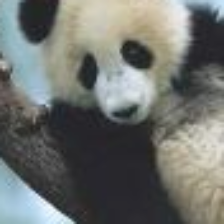
\includegraphics[width=.22\columnwidth]{adversarial-examples/panda_577.png} &%
			\centering\arraybackslash%
			$\centering +\ \epsilon \cdot$ &%
			
\includegraphics[width=.22\columnwidth]{adversarial-examples/nematode_082.png} &%
			$\centering =$ & %
			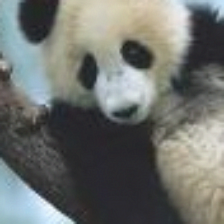
\includegraphics[width=.22\columnwidth]{adversarial-examples/gibbon_993.png} \\
			$\centering \vec x$     &%
			& $\sgn\del{\nabla_{\vec x} L(y,h(\vec x))}$ & & $\tilde{\vec x}$ \\
			\emph{panda} (0.577) & & & & \emph{gibbon} (0.993) 
		\end{tabular}
	}
	\caption{Generation of an adversarial example with FGSM, a single step attack. Italic words and numbers represent classes and confidences. The images are from \citet{Goodfellow:2014:EHAE}.}
	\label{fig:fgsm-adversarial-example}
\end{figure}

\paragraph{Transferability} An interesting property is that adversarial examples generated for one model are often misclassified by other models and models trained on different datasets, i.e. they generalize across models and datasets \citep{Szegedy:2013:IPNN}. This property of adversarial examples is called transferability. This suggests that most state-of-the art deep models are similarly biased. More analysis of transferebility can be found in \citet{Papernot:2016:TMLPBBAAS,Liu:2016:DTAEBBA,Tramer:2017:STAE}. 

\paragraph{Universal perturbations} \citet{Moosavi-Dezfooli:2016:UAP} have observed that there exist perturbations that can reliably produce adversarial examples when added to almost any input and hypothesize that they exploit geometric correlations between different parts of decision boundaries. 

\paragraph{Boundary tilting} \citet{Tanay:2016:ABTPPAE} hypothesize that adversarial examples exist when the decision boundary lies close to the submanifold of sampled data. They suggest that adversarial examples might be occurring along low-variance directions of the data where it is close to the manifold and that robustness could be improved with regularization. This is illustrated in figure \ref{fig:tanay-boundary-tilting}.

\begin{figure}[htbp!]
	\begin{center}
		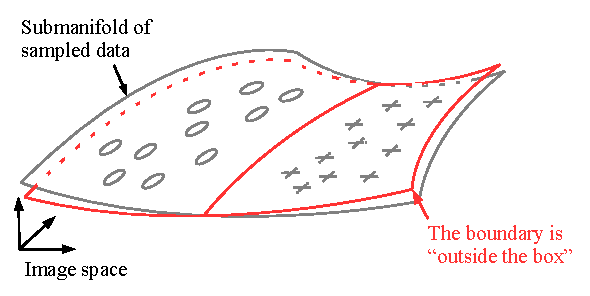
\includegraphics[width=\columnwidth]{figures/adversarial-examples/tanay-newPerspective.pdf}
	\end{center}
	\caption{An illustration of boundary tilting from \citet{Tanay:2016:ABTPPAE}.}
	\label{fig:tanay-boundary-tilting}
\end{figure}

\paragraph{High-dimensional space manifold geometry} \citet{Gilmer:2018:AS} hypothesize that the existence of adversarial examples could be a naturally occurring result of the geometry of high-dimensional data manifolds. For a simple dataset with two classes consisting of examples from a pair of high-dimensional concentric spheres, they have observed that most random points in the data distribution are both correctly classified and close to a misclassified point. The authors have also given negative evidence on the hypothesis that adversarial examples are off the data manifold by showing that \textit{on-manifold} adversarial examples can exist as well.

\paragraph{Adversarial examples of generative models} Adversarial examples are not just a phenomenon related to discriminative models. They have been found to exist for some generative models as well \citep{Goodfellow:2014:EHAE,Kos:2018:AEGM}. An example is shown in figure \ref{fig:vae-gan-targetad-face}.

\begin{figure}[htbp!]
	\begin{center}
		\raisebox{-0.5\height}{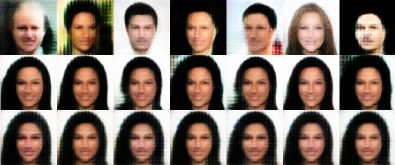
\includegraphics[scale=0.6]{figures/adversarial-examples/kos-exp11-faces-summary.png}}
		~
		\raisebox{-0.5\height}{
\includegraphics[scale=0.075]{figures/adversarial-examples/kos-exp11-faces-target-reconstruction.png}}
	\end{center}
	\caption{Reconstruction outputs for targeted attacks on a VAE-GAN model from \citet{Kos:2018:AEGM}. The rows represent of original image reconstructions (top), reconstructions of adversarial examples generated using an attack in latent space (middle) and a VAE-loss attack (bottom). The target reconstruction is on the right.}
	\label{fig:vae-gan-targetad-face}
\end{figure}

%\paragraph{Adversarial reprogramming.}

\paragraph{True ambiguity of adversarial examples of robust classifers}
Qualitative assesment of adversarial examples of robust classifiers suggest that they \textit{understand data} much better. Their adversarial examples really are ambigous, i.e. generated perturbations don't look like noise but are semantically meaningful to humans \citep{Tsipras:2018:RMBOA,Li:2019:AGCMRAA}.  This is illustrated in figures \ref{fig:tsipras-robust-adversarial-examples} and \ref{fig:li-gfz-adversarial-examples-mnist}. An interesting observation is that adversarially trained discriminative classifiers together with an iterative attack can interpolate between and generate quite realistic examples. \citet{Tsipras:2018:RMBOA} suggest a connection between the the saddle point problem of adversarial training and GAN training \citep{Goodfellow:2014:GAN}.

\begin{figure}[htbp!]
	\begin{center}
		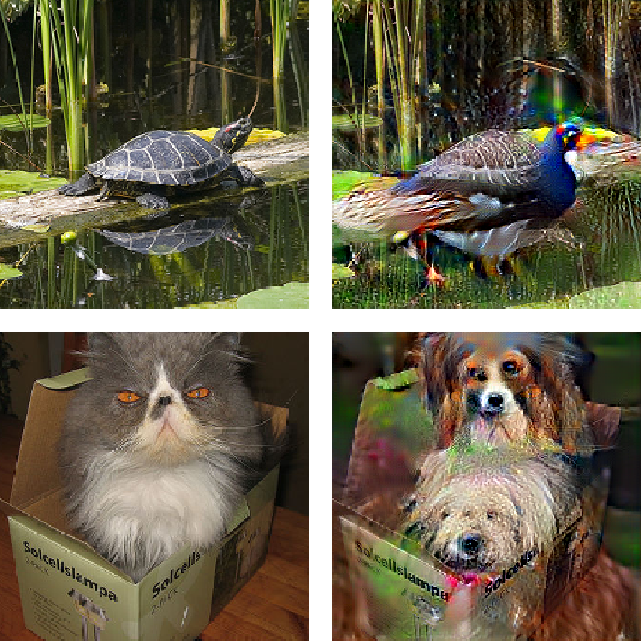
\includegraphics[width=0.85\columnwidth]{figures/adversarial-examples/tsipras-turtle-bird-cat-dogs}
	\end{center}
	\caption{Original images and adversarial examples generated with a large perturbation using an iterative non-targeted attack on an adversarially trained Restricted ImageNet \citep{Tsipras:2018:RMBOA} classifier from \citet{Tsipras:2018:RMBOA}.}
	\label{fig:tsipras-robust-adversarial-examples}
\end{figure}

\begin{figure}[htbp!]
	\begin{center}
		\raisebox{-0.5\height}{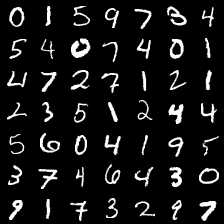
\includegraphics[scale=0.65]{figures/adversarial-examples/li-data_clean.png}}
		\
		\raisebox{-0.5\height}{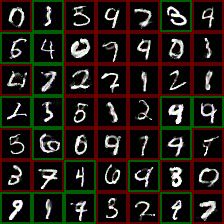
\includegraphics[scale=0.65]{figures/adversarial-examples/li-bayes_A_cw_adv.png}}
	\end{center}
	\caption{Clean images (left) and adversarial examples generated using an iterative non-targeted attack on a generative MNIST \citep{LeCun:2015:DL} classifier with the factorization $\p(\vec z)\p(\vec y\mid\vec z)\p(\vec x\mid\vec z,\vec y)$ (right) from \citet{Li:2019:AGCMRAA}. The adversarial examples marked in green are successful.}
	\label{fig:li-gfz-adversarial-examples-mnist}
\end{figure}

Further interesting phenomena and hypotheses related to the nature of adversarial examples, adversarial robustness and generalization will be discussed in section \ref{sec:robustness-generalization}.


\section{Finding adversarial examples} \label{sec:finding-adversarial-examples}

Let $\set X$ be the input space,
and $d\in(\set X\times\set X\to \R^+)$ a \textit{distance function} for definining similarity between inputs. 
For each example $\vec x$, 
we can also define its \textit{neighbourhood} as $B_{\epsilon}(\vec x) = \cbr{\vec x'\colon d(\vec x', \vec x) \leq \epsilon}$,
where $\epsilon$ is the maximum distance from the example.

Ideally, the neighbourhood of an example $\vec x$ should be the set of \textit{perceptually similar} examples that all belong to the same class as $\vec x$ (their true class may be at most ambiguous), but it is hard to define such a neighbourhood (as it requires knowing the true model). A practical and common way of defining the neighbourhood function for images is to have $d$ be a $L^p$ distance where $p$ is usually $\infty$ or $2$. Note that, if an example is very near the true class boundary, such a neighbourhood may contain examples belonging to another class. 

\subsection{Attack objectives}

Finding an adversarial example can be defined as a constrained optimization problem of maximizing some loss with respect to the input with the constraint that the input is in the neighbourhood $B_\epsilon(\vec x)$:
\begin{align}
    \tilde{\vec x} = \argmax_{\vec x'\in B_\epsilon(\vec x)} L(y, h(\vec x')) \text{,} \label{eq:non-targeted-loss-attack}
\end{align}
where $y$ is the true label. Let $\hat{h}(\vec x) \coloneqq \argmax_{y} h(\vec x)_\ind{y}$ denote the function that assigns the label with the highest probability to an input.
An objective can also be to find the $\tilde{\vec x}$ closest to $\vec x$ such that the classifier misclassifies it \citep{Moosavi-Dezfooli:2016:DFSAMFDNN}:
\begin{align}
    \tilde{\vec x} = \argmin_{\vec x'\colon \vec x'\in B_\epsilon(\vec x) \land \hat{h}(\vec x') \neq y} d(\vec x', \vec x) \text{.} \label{eq:non-targeted-closest-attack}
\end{align}

The described objectives, where it only matters that the adversarial example is misclassified, are objectives for \textit{non-targeted adversarial attacks}. There are also \textit{targeted adversarial attacks}, where the objective is to create an adversarial example such that the model classifies it as some desired target. Targeted attack objectives corresponding to equations \eqref{eq:non-targeted-loss-attack} and \eqref{eq:non-targeted-closest-attack} are:
\begin{align}
    \tilde{\vec x} &= \argmin_{\vec x'\in B_\epsilon(\vec x)} L(y_\text{a}, h(\vec x')) \text{,} \label{eq:targeted-loss-attack} \\
    \tilde{\vec x} &= \argmin_{\vec x'\colon \vec x'\in B_\epsilon(\vec x) \land \hat{h}(\vec x') = y_\text{a}} d(\vec x', \vec x) \text{,} \label{eq:targeted-closest-attack}
\end{align}
where $y_\text{a}$ denotes the adversarial target label. The difference in equation \eqref{eq:targeted-loss-attack} is loss minimization and the adversarial target label instead of the true label. The difference in equation \eqref{eq:targeted-closest-attack} is the condition that the predicted labels equals the adversarial target instead of differing from the true label.

Non-targeted adversarial examples can also be generated without knowledge of the true label. Instead of the true label $y$, the predicted label $\hat{h}(\vec x)$ can be used in equations \eqref{eq:non-targeted-loss-attack} and \eqref{eq:non-targeted-closest-attack}. Such adversarial examples are called \textit{virtual adversarial examples}.
\citet{Miyato:2017:VATRMSSSL,Kurakin:2016:AMLS} propose the following attack objective for use in semi-supervised learning:
\begin{align}
    \tilde{\vec x} = \argmin_{\vec x'\in B_\epsilon(\vec x)} D((\rvar y\mid \vec x, \vec\theta), (\rvar y\mid \rvec x = \vec x', \vec\theta)) \text{,}
\end{align}
where $D$ is some non-negative function that represents distance between distributions.

For adversarial training, non-targeted attacks should be preferred due to the \textit{label-leaking} phenomenon \citep{Kurakin:2016:AMLS} where the learned classifier can overfit to adversarial examples and perform better on them than on natural examples, especially with attacks with a small number of iterations. For robustness evaluation with datasets that have many similar classes, non-targeted attacks can too easily fool the classifier and targeted attacks give more meaningful evaluation results \citep{Athalye:2018:OGGFSS}.

\subsection{Common attacks}

Being that finding adversarial examples is a constrained optimization problem, general gradient-based and black-box optimization algorithms can be used for attacks. Additionally, sometimes techniques specific to some potential defense and machine learning algorithm have to be used.

Some commonly known gradient-based attacks for finding adversarial examples are the following (using the notation from section \ref{sec:finding-adversarial-examples}):
\begin{soliditemize}
	\item Box-constrained L-BFGS -- \citet{Szegedy:2013:IPNN} propose to minimize $c\enVert{\vec x -\tilde{\vec x}}_2^2+L(y,h(\tilde{\vec x}))$ with the constraint $\tilde{\vec x}\in\intcc{0,1}$ with L-BFGS, a quasi-Newton optimization method. $c$ is a number obtained via line-search that yields adversarial examples of minimum distance.
	\item Fast gradient sign method (FGSM) -- an attack proposed by \citet{Goodfellow:2014:EHAE} that requires a single gradient computation:
	\begin{align}
	\tilde{\vec x} = \vec x + \epsilon\nabla_{\vec x} L(y,h(\vec x)) \text{,}
	\end{align} 
	where $\epsilon$ is the $L^\infty$-norm of the perturbation. For $L^2$-constrined perturbations, \citet{Miyato:2017:VATRMSSSL} propose $L^2$ normalization instead of the sign function.
	\item DeepFool -- an iterative non-targeted attack proposed by \citet{Moosavi-Dezfooli:2016:DFSAMFDNN} that in each step finds the optimal solution to a linear approximation of a loss in the $L^2$ ball $B_\epsilon(\vec x)$ using the gradient in the current adversarial input. It is faster and finds smaller perturbations than L-BFGS and stronger than FGSM.
	\item Projected gradient descent (PGD) \citep{Madry:2017:TDLMRAA} or basic iterative method (BIM) \citep{Kurakin:2016:AEPW} -- an iterative gradient-based algorithm with random initialization \citep{Madry:2017:TDLMRAA} of the perturbation from within the $B_\epsilon(\vec x)$ at the start and steps in the direction of the gradient sign:
	\begin{equation} \label{eq:pgd}
	\tilde{\vec x}_i = \Pi_{B_\epsilon(\vec x)} \del{\tilde{\vec x}_{i-1} + \alpha\sgn\del{\nabla_{\tilde{\vec x}_{i-1}} L(y,h(\tilde{\vec x}_{i-1}))}} \text{.}
	\end{equation}
	$\alpha$ is the step size, and $\Pi_{B_\epsilon(\vec x)}$ is the projection into the $L^p$ $\epsilon$-ball around $\vec x$.
	\item Carlini-Wagner (CW) attacks -- \citet{Carlini:2017:TERNN} propose attacks with similar minimal perturbation objectives as \citet{Szegedy:2013:IPNN} and \citet{Moosavi-Dezfooli:2016:DFSAMFDNN}. They modify the loss function and, to enable unconstrained optimization, they introduce change of variables $\vec\delta=\frac{1}{2}\del{\tanh\del{\vec w} + \cvec 1} - \vec x$, which limits the perturbation $\vec\delta$ to the interval $\intcc{0,1}$. With the PGD (BIM) attack, it is currently probably one of the 2 strongest attacks.
\end{soliditemize}


\section{Improving adversarial robustness}

There are different approaches (\textit{defenses}) trying to improve adversarial robustness, most of which have been shown to actually be non-robust, but had appeared robust because they intentionally or unintentionally caused attacks that they were evaluated on to be unable to find adversarial examples \citep{Carlini:2017:AEANEDBTM,Athalye:2018:OGGFSS,Uesato:2018:ARDEAWA,Carlini:2017:TERNN}. Thus, it is important to put as much effort as needed to correctly evaluate robustness, i.e. get an as low as possible upper bound on robustness. \citep{Carlini:2019:OEAR} is a recent helpful overview on evaluation of robustness. 

A broad overview of many defenses can be found in \citet{Serban:2018:AECCP}. To give a few examples, some approaches use generative models to approximately project inputs to a learned data manifold (e.g. \citet{Samangouei:2018:DGPCAAAUGM}), some approaches are based on limiting the Lipschitz constant of the model to limit sensitivity to small input perturbations by regularization and model modification (e.g. \citet{Qian:2018:L2NNN}), some research is looking into ways of guaranteeing robustness (e.g. \citet{Cohen:2019:CARRS}).

\subsection{Adversarial training and empirical adversarial risk}

The only defense currently believed to be effective according to \citet{Athalye:2018:OGGFSS} is adversarial training \citep{Goodfellow:2014:EHAE} with a strong attack \citep{Madry:2017:TDLMRAA}, where the model is trained on adversarial examples as well as natural examples.

\citet{Madry:2017:TDLMRAA} define what can be called \textit{empirical adversarial risk} by allowing the worst-case attack to modify each the input in the empirical risk expression:
\begin{align}
R_\text{EA}(h,\set D) \coloneqq \E_{(\vec x, y)\sim p_{\set D}} \del{\max_{\tilde{\vec x}\in B_\epsilon(\vec x)} L(y,h(\tilde{\vec x}))} \text{.}
\end{align}
They propose PGD for the attack during training and PGD with as large a number of iterations as necessary to approximate the worst-case adversary, i.e. get a better upper bound on robustness.

Still, adversarially trained models are not robust to attacks with weaker constraints than those used for training \citep{Schott:2018:TDFARNNMM}. Furthermore, because adversarial examples are generated and robustness is evaluated according to the practical definition of an adversarial example and using $L^p$ distance as a non-ideal approximation of perceptual similarity, performance is affected \citep{Madry:2017:TDLMRAA,Tsipras:2018:RMBOA} and there can exist misclassified examples among which are \textit{invariance-based} adversarial examples \citep{Jacobsen:2019:EEICNBAR}.

%Empirical and theoretical results show that improving robustness seems to be a problem that requires more model capacity and causes a reduction of performance on natural data \citep{Madry:2017:TDLMRAA,Tsipras:2018:RMBOA}.


\section{Adversarial robustness and generalization} \label{sec:robustness-generalization}

Based on the practical definition of an adversarial example or similar definitions, experimental \citep{Madry:2017:TDLMRAA,Su:2018:IRTCOACSRDICM} and theoretical evidence \citep{Tsipras:2018:RMBOA} suggests that there is a trade-off between robustness and standard generalization for current models.

Here are some recent discoveries related to adversarial robustness and generalization presented. Robustness to distributional shift and corruptions also seems to be quite relevant \citep{Gilmer:2019:AENCTEN,Hendrycks:2019:BNNRCCP}, but it will not be discussed here.

\subsection{A trade-off between robustness and generalization}

\citet{Madry:2017:TDLMRAA,Su:2017:OPAFDNN,Tsipras:2018:RMBOA} and others have empirically observed that adversarial robustness with current algorithms requires more capacity and negatively affects generalization. \citet{Su:2017:OPAFDNN} have observed that older convolutional architectures with no shortcut connections, like AlexNet \citep{Krizhevsky:2012:ICDCNN} and VGG \citep{Simonyan:2014:VDCNLSIR} seem to be inherently more robust than architectures like ResNet \citep{He:2015:DRLIR}, DenseNet \citep{Huang:2016:DCCN} and MobileNet \citep{Howard:2017:MECNNMVA} and NASNets \citep{Zoph:2018:LTASIR} with standard training. \citet{Madry:2017:TDLMRAA} has observed that with adversarial training, more model capacity is required and natural test set performance is reduced. Furthermore, \citet{Tsipras:2018:RMBOA} have, based on the practical definition of an adversarial example, theoretically demonstrated an aspect of the trade-off. Another reason that affects performance suggested by them is that salient features might be harder to learn and that algorithms rely on highly predictive but \textit{non-robust} features.

\subsection{Non-robust features}

Based on some ideas from \citet{Tsipras:2018:RMBOA},  \citet{Ilyas:2019:AENBTF} propose an interesting and experimentally well supported hypothesis on the nature of features that well-generalizing non-robust classifiers learn. They show that existence of adversarial examples can be directly attributed to existence of  non-robust features, "features derived from patterns in the data that are highly predictive but brittle and incomprehensible to humans". 

They demonstrate the predictiveness of non-robust features by: 
\begin{solidenumerate}
	\item constructing a dataset $\set D_\text{NR}$ where approximately the only useful features are non-robust features by turning inputs of the original dataset $\set D$ into adversarial examples for a classifier that was trained standardly and relabeling them with the adversarial label,
	\item training a new classifier on the non-robust dataset $\set D_\text{NR}$,
	\item testing the new classifier on the original test set where it achieves performance close to the original classifier and lower robustness.
\end{solidenumerate}

In another experiment, they try to remove non-robust-features from inputs with the help of an adversarially trained classifier. A new classifier trained on the dataset with removed non-robust features achieves a bit lower performance and robustness not as high as the adversarially trained classifier but quite significant compared to the standardly trained classifier. Results of these experiments with the CIFAR-10 dataset \citep{Krizhevsky:2009:LMLFTI} are shown in figure \ref{fig:iliyas-experiment-results}.

\begin{figure*}[htbp!]
	\centering
	\begin{subfigure}[b]{0.45\textwidth}
		\centering
		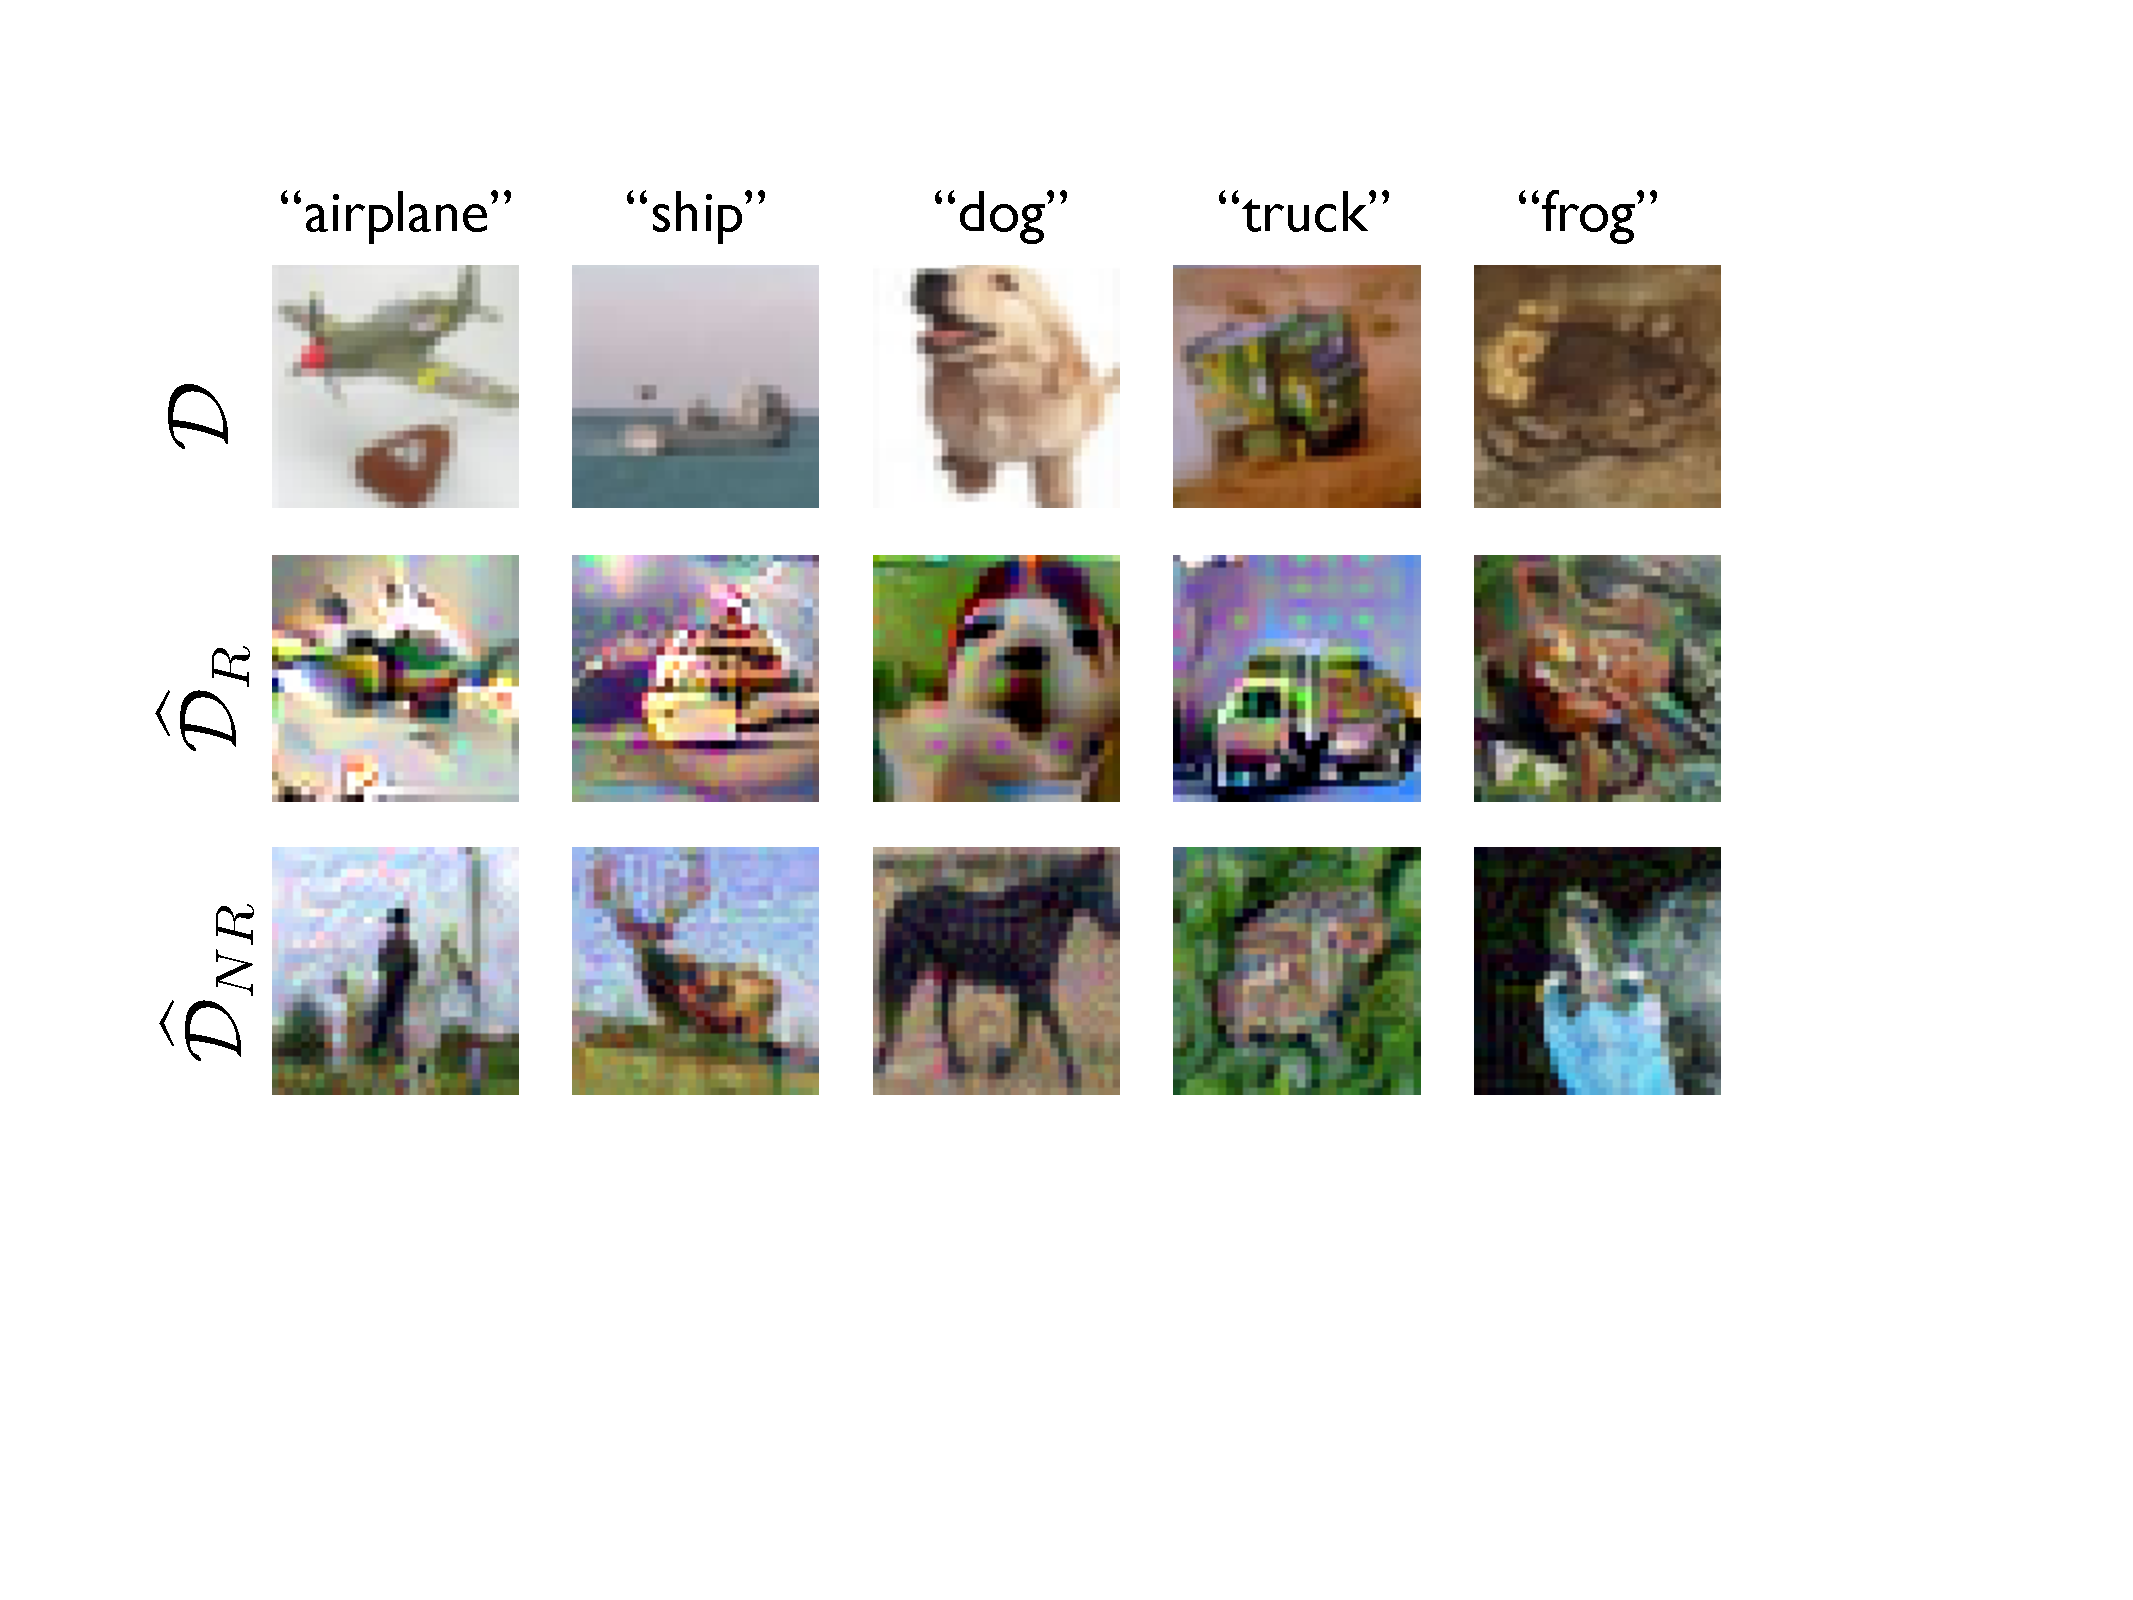
\includegraphics[width=1.0\textwidth]{figures/adversarial-examples/ilyas/cifar_datasets.pdf}
		\vfill\null
		\caption{}
		\label{fig:robust_inputs}
	\end{subfigure}
	\hfill
	\begin{subfigure}[b]{0.5\textwidth}
		\centering
		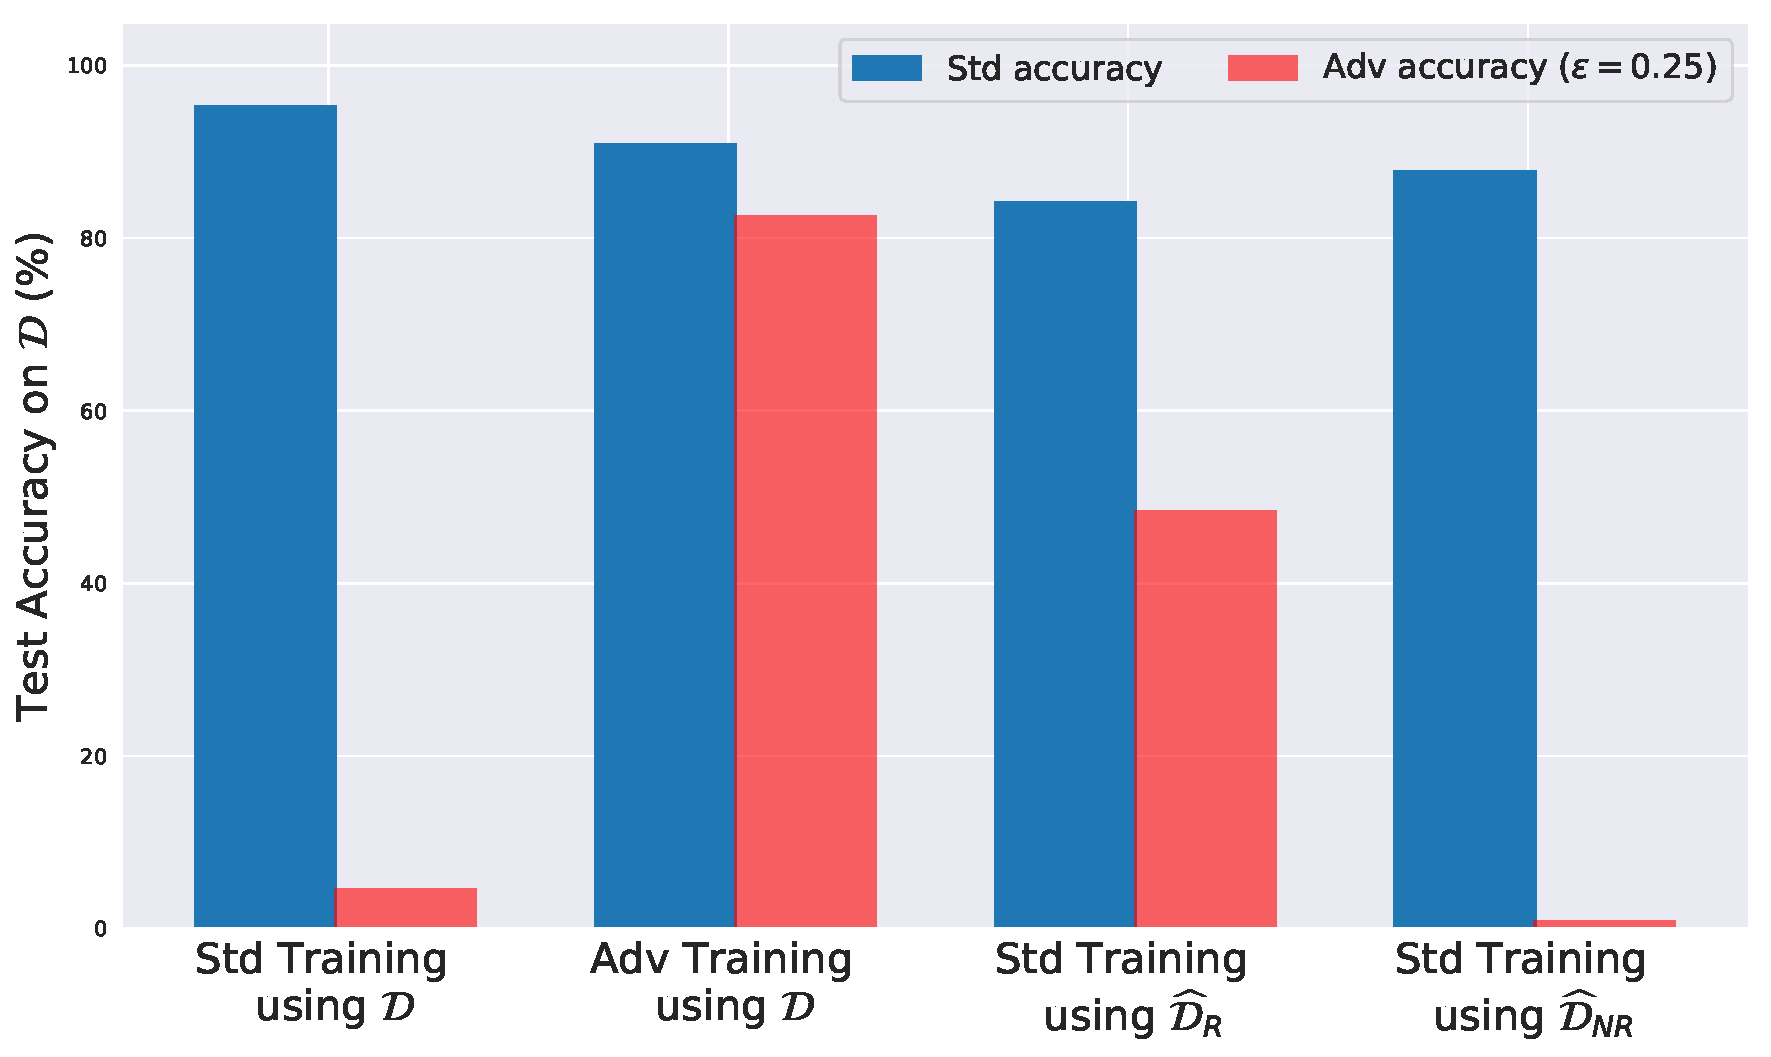
\includegraphics[width=\textwidth]{figures/adversarial-examples/ilyas/CIFAR_res.pdf}
		\caption{}
		\label{fig:robustify_cifar}
	\end{subfigure}
	\caption{
		(a) Random samples from variants of the
		CIFAR-10 training set:
		the original training set; 
		the \textit{robust training set} $\set D_\text{R}$, restricted to features used by a
		robust model; and
		the \textit{non-robust training set} $\set D_\text{NR}$, restricted to
		features relevant to a standard model (labels appear incorrect to humans).
		(b) Standard and robust accuracy on the CIFAR-10
		test set ($\set D$) for models trained with standard training, adversarial training, and standard training on datasets $\set D_\text{R}$ (robust) and $\set D_\text{NR}$ (non-robust). Adapted from \citet{Ilyas:2019:AENBTF}.}
	\label{fig:iliyas-experiment-results}
\end{figure*}

\subsection{Training with on-manifold adversarial examples}

\citet{Stutz:2018:DARG} challenge the hypothesis that there is a trade-off between robustness and generalization. They hypothesize that most adversarial examples come from directions orthogonal to the learned class manifolds and that training adversarial examples (as per a definition similar to definition \ref{def:ae-consistent}) limited to the known or learned class manifolds (on-manifold adversarial examples) can improve generalization. They conduct experiments with a synthetic dataset with known class-invariant transformations and datasets with small images that support the hypothesis that generalization can be improved with adversarial training with on-manifold adversarial examples.

Class manifolds to which adversarial examples are restrited and on-manifold and off-manifold adversarial examples are illustrated in figure \ref{fig:stutz-illustration}.

\begin{figure}[htbp!]
	\begin{center}
		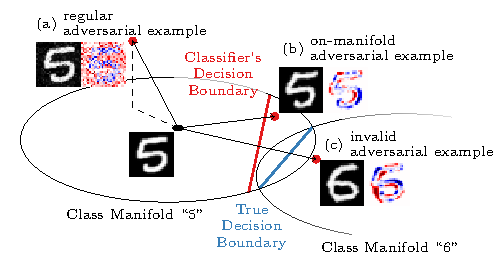
\includegraphics[width=\columnwidth]{figures/adversarial-examples/stutz-introduction_b.pdf}
	\end{center}
	\caption{An illustration by \citet{Stutz:2018:DARG} of class manifolds (classes "5" and "6") with a regular (off-manifold) adversarial example and an on-manifold adversarial example.}
	\label{fig:stutz-illustration}
\end{figure}

In one of the experiments \citet{Stutz:2018:DARG} construct a synthetic dataset with a known manifold (geometric transformations of letters) in order to be able to generate exactly on-manifold adversarial examples by modifying parameters of the geometric transformations. With this dataset, they succeed in improving generalization and on-manifold robustness\footnote{By the authors' definition of an adversarial example, which is similar to the consistent definition (definition \ref{def:ae-consistent}), except for that there is no closeness constraint, making it equivalent to the definition of a misclassified example, on-manifold robustness essentially boils down to generalization.} with adversarial training.

In other experiments they use EMNIST \citep{Cohen:2017:EMNIST}, FashionMNIST \citep{Xiao:2017:FMNIDBMLA} and CelebA \citep{Liu:2015:DLFAW}. In order to better approximate class manifolds and disable leaving the manifold of a class when an adversarial example is generated for adversarial training, they first train one variational autoencoder (VAE-GAN) per class. They perform training and evaluation analogously to the experiment with synthetic data by allowing the attack to perturb the latent representation of the autoencoder corresponding to the correct class. They measure positive correlation between robustness to on-manifold adversarial examples and generalization. They observe worse quality of on-manifold adversarial examples for the more complex dataset CelebA due to worse approximation quality of their VAE-GAN-s.


\section{Conclusion}

This paper presents an overview of ideas related to the existence adversarial examples, hypotheses on their existence and some of their properties. It describes general principles regarding adversarial attacks, defenses and robustness evaluation and presents examples of such algorithms. Finally, some recent discoveries and hypotheses regarding the relation between robustness and generalization are explored. Some recent results \citep{Stutz:2018:DARG} suggest that finding ways of improving both robustness generalization might be an interesting research direction to explore.


\bibliography{bibliography}
%\bibliographystyle{plainnat} 
%\bibliographystyle{ieeetr}
\bibliographystyle{IEEEtranN}

\end{document}
